\documentclass[letterpaper, 11pt]{article}
\usepackage{amsmath,amssymb,amsthm,fullpage,placeins,textcomp, multirow, subcaption, listings, empheq,esint, bm, hyperref, enumitem}
\usepackage[noend]{algpseudocode}
\usepackage[]{algorithm}
\usepackage{booktabs}
\usepackage{tikz}
\usepackage{tkz-berge}
\usepackage{array}


\usepackage[letterpaper, margin=1in]{geometry}
\newcolumntype{L}[1]{>{\raggedright\let\newline\\\arraybackslash\hspace{0pt}}m{#1}}
\newcolumntype{C}[1]{>{\centering\let\newline\\\arraybackslash\hspace{0pt}}m{#1}}
\newcolumntype{R}[1]{>{\raggedleft\let\newline\\\arraybackslash\hspace{0pt}}m{#1}}


\begin{document}
\title{CS/EE 144 Pandemaniac Report}
\author{Team kraftwerk \\Fabian Boemer, Jessica Li}
\date{\today}
\maketitle


\textbf{TODO:}
parallel computations? Jessica's things (spectral clustering?), visualizations. Descriptions of different centralities and why they wold be promising. Intro/Conclusion


\section{Introduction and Overview}
\subsection{Introduction}
We used networkx \cite{networkx}

\textbf{TODO}

\subsection{Counterexample}
In some cases, a set of initial colorings may result in a game which fails to converge. Consider, for example, the complete bipartite graph, $K_{m,n}$, $m,n \geq 2$ with disjoint nodesets $U, V$ and initial colorings red $R= U$, blue $B=V$. At each timestep, time $t$, the nodes in $A$ will convert the of nodes in $V$. Meanwhile, the nodes in $B$ will convert the nodes in $U$. There are no edges between colored nodes initially, and this property remains through each iteration. So, the colorings will always alternate between the bipartite sets. Figure \ref{fig:converge} shows the behavior of this game, which fails to converge.
  
\begin{figure}[h!]   
\begin{center}
\tikzstyle{every node}=[circle, draw, fill=black, minimum width=10pt]

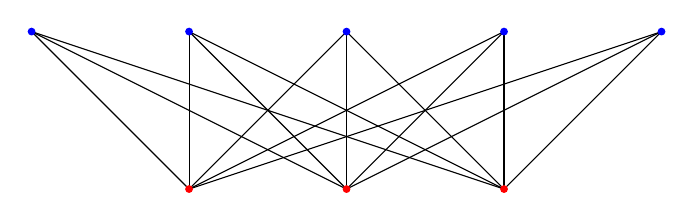
\begin{tikzpicture}
\foreach \x in {-2,-1,0,1,2}
	\foreach \y in {-1,0,1}{
		\draw (2*\y,0) -- (2*\x,2);
	}
	\foreach \x in {-2,-1,0,1,2}{
		\node[blue,circle,inner sep=1pt,fill] at (2*\x,2) {};
	}
	\foreach \x in {-1,0,1}{
		\node[red,circle,inner sep=1pt,fill] at (2*\x,0) {};
	}
\end{tikzpicture}
\caption{Graph at $t\mod 2 = 0$}

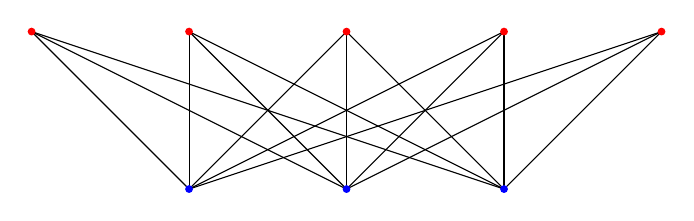
\begin{tikzpicture}
\foreach \x in {-2,-1,0,1,2}
	\foreach \y in {-1,0,1}{
		\draw (2*\y,0) -- (2*\x,2);
	}
	\foreach \x in {-2,-1,0,1,2}{
		\node[red,circle,inner sep=1pt,fill] at (2*\x,2) {};
	}
	\foreach \x in {-1,0,1}{
		\node[blue,circle,inner sep=1pt,fill] at (2*\x,0) {};
	}
\end{tikzpicture}
\caption{Graph at $t\mod 2 = 1$}
\label{fig:converge}
\end{center}

\end{figure}

\section{Visualization}
Visualization was an important component of this project, especially for understanding how seed node selection propogated through the graph. We explored several built-in and custom visualizations through the networkx package. One critertion for visualization was maintaining a consistent A circular layout was not instructive and nodes were too close together. We implemented a custom grid layout, as in Figure \ref{fig:visualization}. The grid layout failed to capture the structure of the graph, but was useful for viewing the progress of cascades.
\par
To visualize the structure of the graph at a single timepoint, we used networkx's `spectral layout', which uses Hooke's law with force proportional to node degree to place nodes. Figure \ref{fig:visualization} shows a coloring of graph clusters, which is useful for understanding general graph structure.

\begin{figure}[h]
\begin{center}
\begin{subfigure}{.49\textwidth}
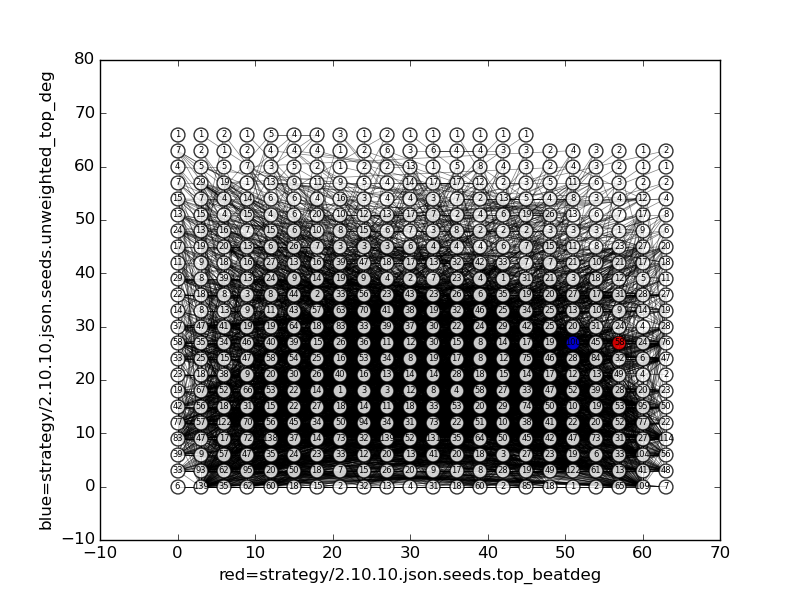
\includegraphics[width=\textwidth]{{day1_figs/2.10.10.json_iter_1}.png}
\caption{Grid layout}
\end{subfigure}
\begin{subfigure}{.49\textwidth}
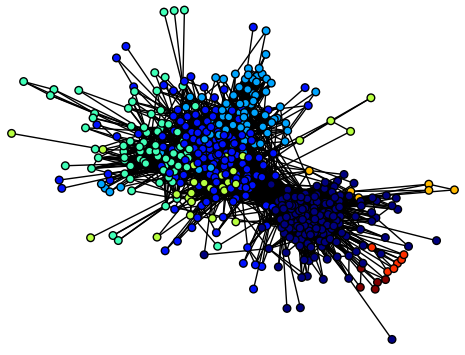
\includegraphics[width=\textwidth]{{day5_figs/2.10.32}.png}
\caption{Spectral layout of graph clusters.}
\end{subfigure}
\caption{Visualization of graphs 2.10.31 and 2.10.32}
\label{fig:visualization}
\end{center}
\end{figure}
\par
We only used visualization for offline learning. A more complete approach might use human input to visually select important nodes.


\section{Algorithms}
\subsection{Day 1: Cancellation}
The first approach was a naive cancellation approach designed to beat TA-degree. Algorithm \ref{alg:cancellation} gives the pseudocode for the cancellation approach.
\begin{algorithm}
\caption{Cancellation Algorithm}
\label{Cancellation}
\begin{algorithmic}[1]
\Procedure{Cancellation}{$G$, $n$}
\State Order the nodes by degree centrality
\State Select the $n-1$ nodes with highest degree centrality
\State Select the previously-unselected node adjacent to the vertex of highest-degree.
\State \textbf{return} selected nodes.
\EndProcedure
\end{algorithmic}
\label{alg:cancellation}
\end{algorithm} \\
Time constraints prevented us from testing this strategy before the Day 1 run. We visualized the results from the Day 1 run against TA-degree, and visualized each iteration in Figure \ref{fig:cancellation}.

\begin{figure}[h!]
\begin{center}
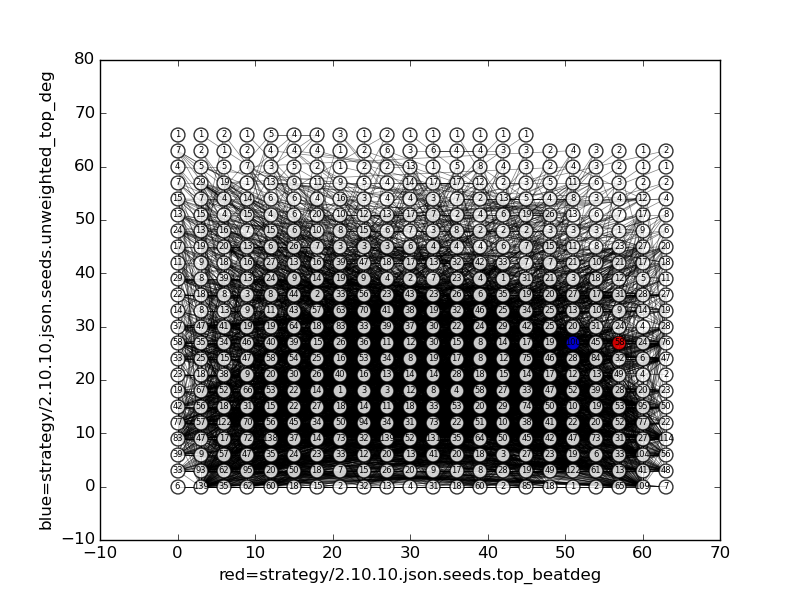
\includegraphics[width=.49\textwidth]{{day1_figs/2.10.10.json_iter_1}.png}
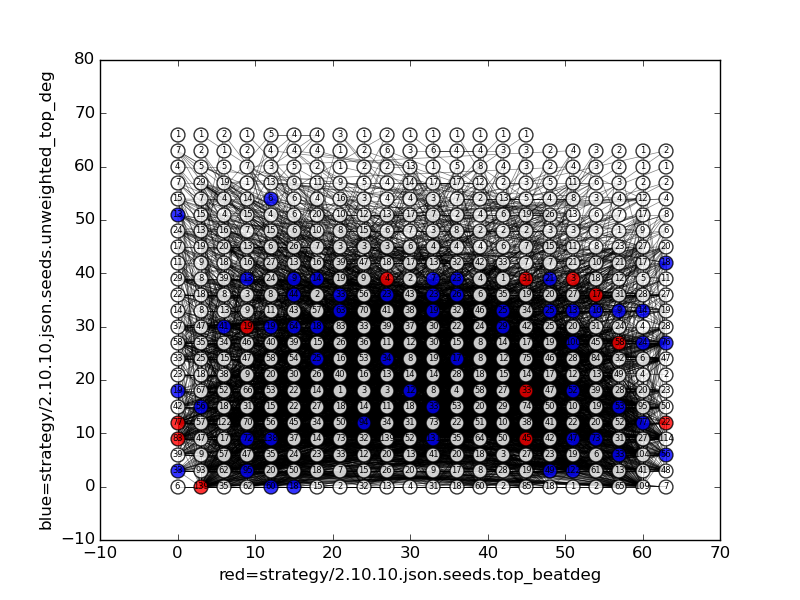
\includegraphics[width=.49\textwidth]{{day1_figs/2.10.10.json_iter_2}.png}
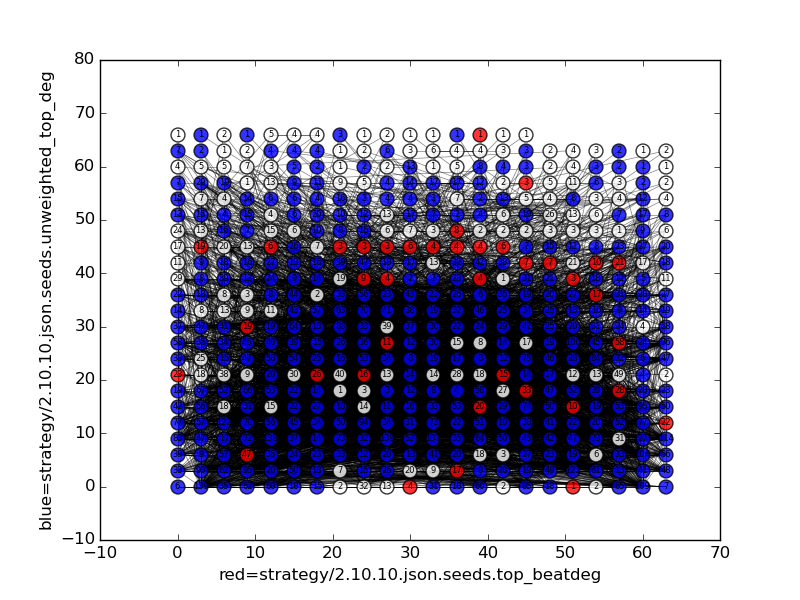
\includegraphics[width=.49\textwidth]{{day1_figs/2.10.10.json_iter_3}.png}
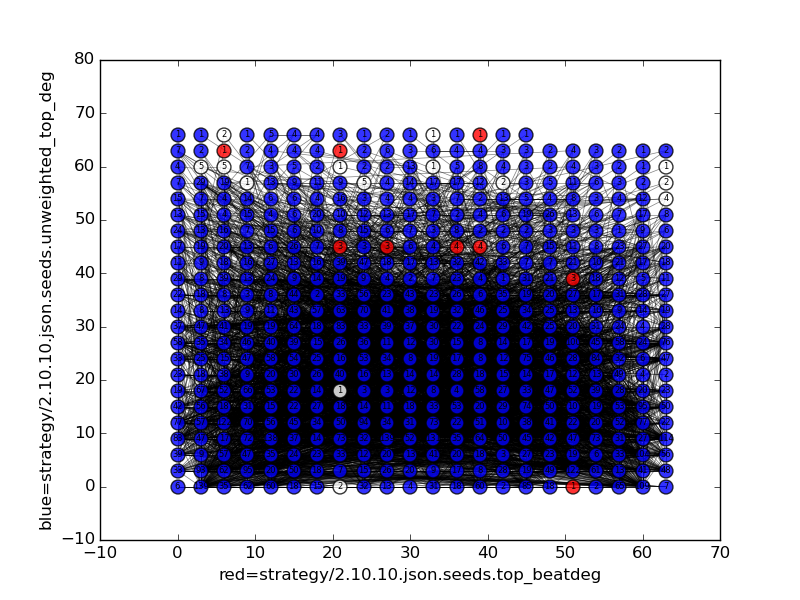
\includegraphics[width=.49\textwidth]{{day1_figs/2.10.10.json_iter_4}.png}
\caption{Results from Day 1 against TA-degree. Our team's nodes are red; the TA's nodes are blue. The numbers in the nodes indicate the node degree.}
\label{fig:cancellation}
\end{center}
\end{figure}
The top-left plot is iteration 1, where we notice only one node of each color is selected, by construction. The top right right is iteration 2, where we see the red node adjacent to the bottom-left corner, with degree 139. So our strategy successsfully claimed the highest-degree node. However, the TA's blue seed node has high degree, and claimed several blue nodes. Then, at iteration 3, we see the highest-degree node failed to convert many nodes. The TA already has spread to enough nodes that converting any new nodes is difficult. By iteration 4, it is clear the blue nodes have won. Thus, our cancellation approach is too slow; the controlling the highest-degree node at iteration 2 is not enough to win against TA-degree.
\par
As simulated, we did not beat TA-degree on day 1. We did, however, beat TA-fewer. This is not unexpected, since the $n-1$ nodes with high degree centrality are a decent selection of important nodes.

\subsection{Day 2: Centrality Measures}
On day 2, we focused on developing a strategy to beat TA-degree. We explored several different measures of centrality, including betweeness, current flow betweenness (cfbet), closeness, and eigenvector centrality. First we tried taking top $n$ most-important nodes, as ranked by each centrality measure, excluding degree-centrality since TA-degree uses degree centrality. We modified `sim.py' to simulate each selction strategy against TA-degree. Table \ref{table:day2} shows the results of our simulations

\begin{table}\centering
\begin{tabular}{cccccc}
Day & Graph & Centrality measure & Strategy count & TA-degree count & Ratio \\ \hline
\toprule
\multirow{1}{*}{1}
& 2.10.10 & betweenness & 18 & 482 & 0.04 \\
& 2.10.10 & cfbet & 491 & 9 & 0.99 \\ 
& 2.10.10 & closeness & 386 & 113 & 0.77 \\
& 2.10.10 & eigenvector & 394 & 106 & 0.79\\ \cmidrule{2-6}

& 2.10.20 & betweenness & 43 & 455 & 0.08 \\
& 2.10.20 & cfbet & 43 & 455 & 0.08 \\ 
& 2.10.20 & closeness & 452 & 45 & 0.90\\
& 2.10.20 & eigenvector & 429 & 69 & 0.86\\ \cmidrule{2-6}

& 2.10.30 & closeness & 475 & 22 & 0.96\\
& 2.10.30 & eigenvector & 469 & 28 & 0.94\\
\midrule

\multirow{1}{*}{2}
& 2.10.11 & cfbet & 31 & 468 & 0.06\\
& 2.10.11 & closeness & 231 & 263 & 0.47 \\
& 2.10.11 & eigenvector & 239 & 256 & 0.48\\ \cmidrule{2-6}

& 2.10.21 & closeness & 277 & 216 & 0.56 \\
& 2.10.21 & eigenvector & 206 & 283 & 0.42\\ \cmidrule{2-6}

& 2.10.31 & closeness & 35 & 456 & 0.07 \\
& 2.10.31 & eigenvector & 28 & 464 & 0.056 \\
\bottomrule
\end{tabular}
\caption{Summary of local testing results for each centrality measure for Day 2.}
\label{table:day2}
\end{table}


From the Day 1 simulations, we see closeness and eigenvector centrality consistently outperformed TA-degree. For our submission, we set up a local pipeline to generate seeds for current flow betweeness, closeness, and eigenvector centralities, and simulate TA-degree against each centrality measure. We expeceted at least one of the three strategies to beat TA-degree on graph 2.10.11, based on the performances on graphs 2.10.10, 2.10.20, 2.10.30.
\par
Unfortunately, during submission, we simulated narrow losses against TA-degree with closeness and eigevector centralities, with a heavy loss with current-flow betweenness. The simulation was correct, as we failed to beat TA-degree.
\par
We spent some time trying to visualize the structure of the graphs. Unforunately, the visualizations produced by networkx's 'spring layout' were inconsistent between successive drawings, and the remaining visualization formats did not expose the structure of the graph. Thus, we used visualization only sparingly from this point forward.
\par
We tried clustering the grpaph using networkx's, ‘k\_components = apxa.k\_components(G)’. For 500-node graphs, the clustering took 129 seconds, which was deemed too long for the 3 minute deadline.

\subsection{Day 3: Monte-Carlo}
Having failed to beat TA-degree, we increased the scope of our approach. We explored several new measures of centrality, and began exploring blending of results. We included Katz centrality and dispersion centrality, \textbf{which are good for what?}
Each of these centrality measures took only a few seconds, we explored a more complete use of our available time through Monte-Carlo simulations. Algorithm \ref{alg:promising} is the pseudocode for this approach.
\par
This is a non-disciminative approach, which does not distinguish between the efficacy of each centrality, nor the complementary advantages of each centrality measure. For example, nodes with high betweenness measure are likely prevent cascades from spreading, while nodes with high closeness centrality spread quickly to all nodes in a cluster. Nevertheless, this approach successfully generated several strategies simulated to win against TA-degree. Having not yet beat TA-more, we varied our final output among the top-10 best-performing strategies simulated to beat TA-more. This provides more variance in the seeding, and makes the seeding more robust against an adverserial TA seeding.
\par
As simulated, we successfully beat TA-degeree with this approach. However, we still failed to beat TA-more.

\begin{algorithm}
\caption{Promising Algorithm}
\begin{algorithmic}[1]
\Procedure{Promising}{$G$, $n$}
\State Order the nodes by degree centrality, eigenvector centrality, Katz centrality, closeness centrality, dispersion centrality.
\State Initialize dictionary $d$ with keys all the nodes and values as 0
\For{each centrality measure}
\For{node in top $n$ ranking}
\State Let $d[\text{node}] += n - $ ranking.
\EndFor
\EndFor
\State Sort $d$ descending by value and choose 12 highest-value nodes as 'promising'
\For{each of $12 \choose 10$ combinations of 10 seed nodes }
\State Simulate the seed against TA-degree
\EndFor
\State Order seeds by number of nodes claimed against TA-degree
\While{Final Seeding not complete}
\For{the top ten seeds ranked by performance}
\State populate Final Seeding with the ten seeds
\EndFor
\EndWhile
\EndProcedure
\State \textbf{return} Final Seeding.
\end{algorithmic}
\label{alg:promising}
\end{algorithm}

\subsection{Day 4: Blending}
We expanded on our idea of blending promising nodes into a more refined approach. We took the $n$ most promising nodes based on degree centrality, betweenness and eigenvector centrality. We reasoned that nodes with high degree centrality would effectively conquer clusters, while nodes with high betweeness would effectively blockade cascasdes from proceeding between clusters. Up to this point, eigenvector centrality performed quite well and was computed very rapidly, so we decided to include the nodes with high eigenvector centrality as well.


\begin{algorithm}
\caption{Hybrid Algorithm}
\begin{algorithmic}[1]
\Procedure{Hybrid}{$G$, $n$}
\State Order the nodes by degree centrality, eigenvector centrality, Katz centrality, closeness centrality, dispersion centrality.
\State Generate the set $s$ of top-$n$ ranked nodes in each centrality measure
\State Generate 100 random selections of $n$ nodes from $s$.
\For{each of 100 seed node selections}
\State Simulate seed nodes against TA-degree with $1.2n$ nodes.
\EndFor
\State \textbf{return} best-performing set of seed nodes.
\EndProcedure
\end{algorithmic}
\label{alg:hybrid}
\end{algorithm}

\textbf{LOCAL RESULTS!?}

On the Day 4 run, we still failed to beat TA-more. Thus, the brute-force generation of `important' nodes failed to quickly cover enough variation in seed nodes to beat TA-more



\subsection{Day 5: Clustering}
On Day 5, we discovered a faster way of partitioning based on the Louvain method \cite{louvain}, and implemented in networkx. This clustering approach was much quicker than the previous approach using ‘k\_components = apxa.k\_components(G)’. The size of the clusters varied from less than 10 to over 100 for a 500-node graph, and were not disjoint. We adapted previous approaches to clustering, described in Algorithm \ref{alg:cluster}.


\begin{algorithm}
\caption{Cluster Algorithm}
\begin{algorithmic}[1]
\Procedure{Hybrid}{$G$, $n$}
\State Cluster $G$ using Louvain method
\For{each cluster $c$}
\State Use promising($c$, $n$) to generate `most-important' node within the cluster.
\EndFor
\For{each of 3 populating strategies}
\State Initialize empty FinalSeeding list
\While{FinalSeeding length less than $n$}
\For{each cluster $c$}
\State Insert most-important node(s) from $c$ not yet in FinalSeeding
\EndFor
\State Simulate FinalSeeding against TA-more Day 4
\EndWhile
\EndFor
\State \textbf{return} best-performing FinalSeeding
\EndProcedure
\end{algorithmic}
\label{alg:cluster}
\end{algorithm}

In line 8, we explored three methods of choosing the number of most-important node(s) selected. For a given cluster $c$, we populate FinalSeeding with the number of nodes proportional to one of:
\begin{enumerate}[label=(\arabic*)]
\item the total degree of nodes in $c$
\item the number of edges in $c$
\item 1 (each cluster has the same number of nodes)
\end{enumerate}

We simulated the results against the nodes picked by TA-more on previous days. Our findings are summarized in Table \ref{table:day5}.
\begin{table}[h!]\centering
\begin{tabular}{ccccc}
Graph & Strategy & Proportion Nodes Claimed & Games won \\ \hline
\toprule
2.10.31 & (1) & 0.04 & 0 \\
2.10.31 & (2) & 0.06 & 1 \\
2.10.31 & (3) & 0.04 & 0 \\
\midrule

2.10.32 & (1) & 0.60 & 47 \\
2.10.32 & (2) & 0.21 & 4 \\
2.10.32 & (3) & 0.21 & 7 \\
\midrule
\bottomrule
\end{tabular}
\caption{Summary of local testing results using clustering approach for Day 5.}
\label{table:day5}
\end{table}



The visualization in Figure \ref{fig:day5} between graphs 2.10.31 and 2.10.32 suggested 2.10.32 was more clearly clustered than 2.10.31, suggesting our approach (1) works well for clustered graphs. This makes sense for clusters of roughly equal size. Nevertheless, we see 2.10.31 has a separate cluster of only 3 nodes, which is likely not worth placing a seed on. In retrospect, perhaps our strategies were placing too much weight on small clusters. Rather, perhaps, we should have chosen only nodes from the largest cluster.
\begin{figure}[h]
\begin{center}
\begin{subfigure}{.49\textwidth}
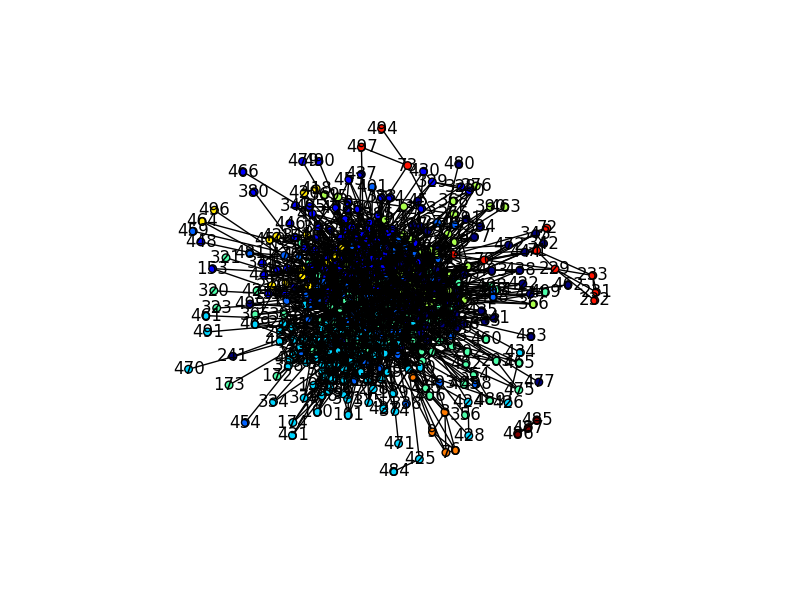
\includegraphics[width=\textwidth]{{day5_figs/2.10.31}.png}
\caption{2.10.31}
\end{subfigure}
\begin{subfigure}{.49\textwidth}
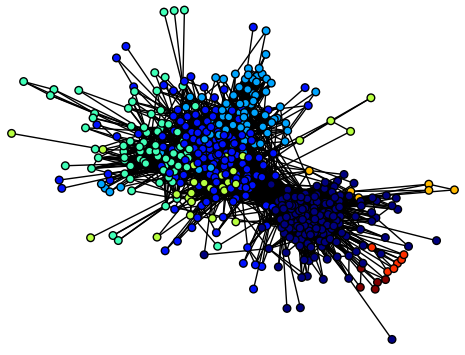
\includegraphics[width=\textwidth]{{day5_figs/2.10.32}.png}
\caption{2.10.32}
\end{subfigure}
\caption{Visualization of graphs 2.10.31 and 2.10.32}
\label{fig:day5}
\end{center}
\end{figure}
\par
In Table \ref{table:graphs} in Section \ref{appendix}, we see graph 2.10.32 has high average and overall clustering coefficient, as compared to graph 2.10.30, and also a higher Louvain modularity. This might suggest our approach (1) might only work well for graphs with these properties.

\par
Under time constraint, we decided to use the number of nodes proportional to the number in each cluster, since this was the only winning approach we discovered. Unfortunately, this failed to beat TA-more.


\section{Conclusion}

\pagebreak
\section{Appendix}\label{appendix}
\begin{table}[h!]\centering
\begin{tabular}{c | C{2.0cm} | C{2.0cm} | C{2.5cm} |C{1.7cm}|C{1.7cm}|C{1.7cm}|C{1.9cm}}
Graph & Average Clustering Coefficient & Overall Clustering Coefficient & Connected Components & Maximal Diameter & Average Diameter & Partitions & 
Louvain Modularity \\ \hline
2.10.30 & 0.44 & 0.28 & 2 & 6 & 2.61 & 7.0 & 0.35\\
2.10.31 & 0.46 & 0.28 & 2 & 7 & 2.65 & 10.0 & 0.34\\
2.10.32 & 0.51 & 0.36 & 1 & 6 & 2.83 & 8.0 & 0.5\\
2.10.33 & 0.47 & 0.3 & 1 & 7 & 2.61 & 12.0 & 0.34\\
2.10.34 & 0.48 & 0.27 & 1 & 7 & 2.83 & 8.0 & 0.47\\ \hline

2.10.20 & 0.42 & 0.29 & 1 & 7 & 2.78 & 9.0 & 0.4\\
2.10.21 & 0.53 & 0.36 & 2 & 7 & 2.87 & 11.0 & 0.48\\
2.10.22 & 0.47 & 0.29 & 1 & 7 & 2.58 & 6.0 & 0.38\\
2.10.23 & 0.47 & 0.3 & 1 & 6 & 2.53 & 6.0 & 0.36\\
2.10.24 & 0.48 & 0.31 & 1 & 6 & 2.64 & 9.0 & 0.36\\ \hline

2.10.10 & 0.48 & 0.31 & 1 & 6 & 2.55 & 7.0 & 0.4\\
2.10.11 & 0.51 & 0.32 & 1 & 8 & 2.68 & 8.0 & 0.33\\
2.10.12 & 0.52 & 0.36 & 1 & 7 & 2.93 & 5.0 & 0.45\\
2.10.13 & 0.5 & 0.33 & 1 & 6 & 2.95 & 9.0 & 0.49\\
2.10.14 & 0.5 & 0.32 & 1 & 6 & 2.75 & 9.0 & 0.46\\
\end{tabular}
\caption{Submission graph information}
\label{table:graphs}
\end{table}

\newpage
\begin{thebibliography}{9}

\bibitem{louvain}
Fast unfolding of communities in large networks, Vincent D Blondel, Jean-Loup Guillaume, Renaud Lambiotte, Renaud Lefebvre, Journal of Statistical Mechanics: Theory and Experiment 2008(10), P10008 (12pp)

\bibitem{networkx}
https://networkx.github.io/

\end{thebibliography}


\end{document}
